\chapter{Deseño}

Neste capítulo explicaremos a arquitectura da plataforma empezando por unha visión xeral da mesma e despois comentando máis en detalle o deseño do servidor e da aplicación Android.



\section{Arquitectura xeral}

A nosa plataforma consta dos seguintes elementos (ver figura~\ref{fig:arq_xeral}):
\begin{itemize}
 \item Servidor base de datos (POIs e percorridos).
 \item  Aplicación Android para visualización e edición de datos.
 \item Sistema de autenticación (GoogleAuth).
  \item Sistema de localización en interiores (Situm).
\end{itemize}


\begin{figure}[tb] 
	\begin{center}
		\includegraphics[width=0.65\textwidth]{figures/arq_xeral}
		\caption{Arquitectura xeral da plataforma Caronte para a guía de museos.}
		\label{fig:arq_xeral}
	\end{center}
\end{figure}



%%%%%%%%
\section{Modelo de datos}


\begin{figure}[tb] 
	\begin{center}
		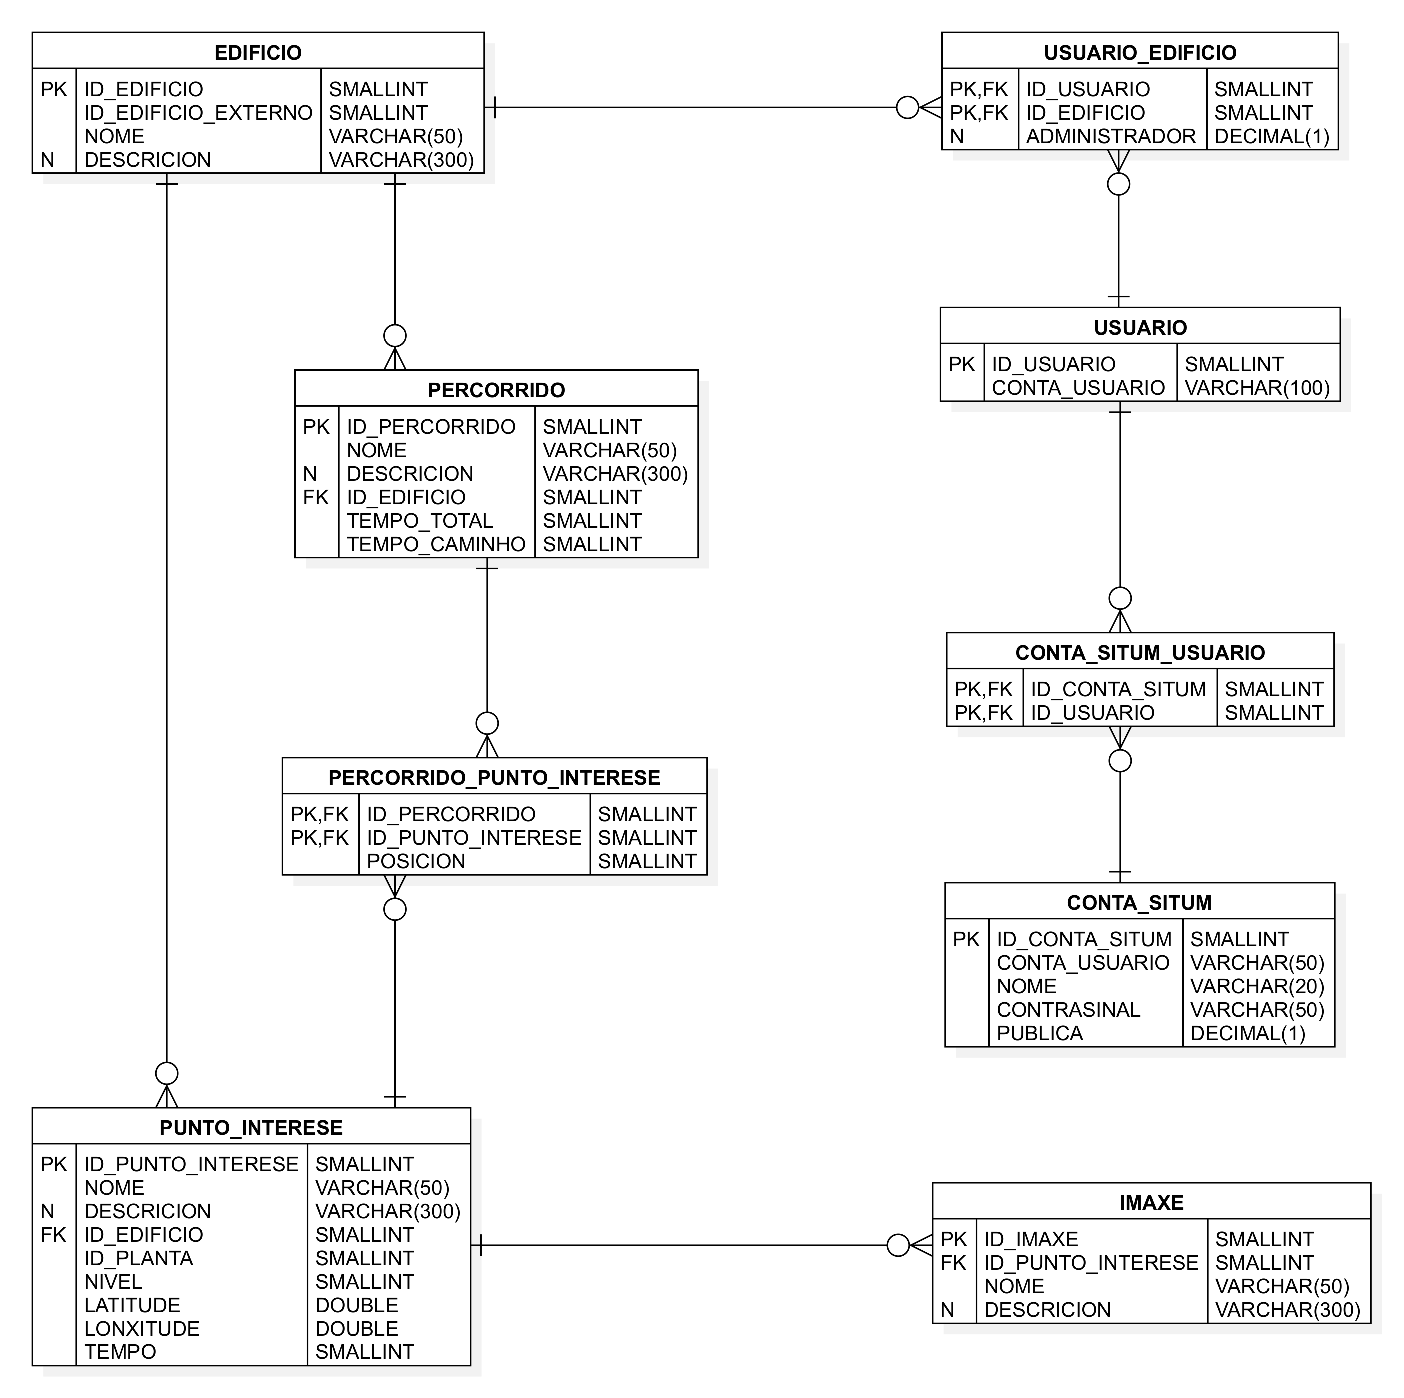
\includegraphics[width=0.95\textwidth]{figures/BD/diagramaEntidadeRelacion}
		\caption{Modelo de datos da plataforma Caronte.}
		\label{fig:modelo_datos}
	\end{center}
\end{figure}


%%%%%%%%
\section{Servidor base de datos}



%%%%%%%%
\section{API rest}


%%%%%%%%
\section{Aplicación Android}


